% !TEX root = ../main.tex

\chapter{Introduction}\label{chapter:introduction}

Urban traffic is hard to describe analytically.\ Millions of daily trips produce congestion patterns that emerge from the interaction of many individual choices, and a policy intervention -- closing an arterial, reducing road capacity, opening a new metro line -- reshapes those patterns through the responses of individual travellers.\ Agent-based simulators such as MATSim handle this kind of question by modelling each traveller's daily activity, mode and route choices, then iterating until the system converges to an approximate user equilibrium~\autocite{horni2016matsim,bonabeau2002agent,railsback2019agent}.\ The price of that fidelity is computational: a single Paris-scale scenario takes more than eight hours on modern hardware~\autocite{natterer2025ml}.\ For a planner who wants to compare a dozen variations of a road-pricing scheme, that cost is prohibitive.

Machine-learning surrogates promise to compress the loop from hours to seconds.\ \textcite{natterer2025ml} showed that Graph Neural Networks (GNNs) are particularly well suited to this task: they exploit the topology of the road network natively while learning per-segment volume responses to capacity changes.\ Their PointNetTransfGAT architecture is the model this thesis builds on.

Accuracy alone is not enough for decision support.\ A model trained on a limited set of scenarios will eventually face inputs unlike anything it has seen, and at that point its predictions can deteriorate without any external indication that something has changed.\ Without uncertainty quantification (UQ), planners cannot separate the reliable predictions from the unreliable ones, and a confident-but-wrong output can drive a poor infrastructure decision.\ This thesis addresses that gap by evaluating Monte Carlo Dropout, deep ensembles, conformal prediction, post-hoc regression $\sigma$-scaling, and several uncertainty-aware training variants on a GNN surrogate for policy-induced changes in traffic volume.\ The empirical work is deliberately constrained to one road network (Paris), one intervention type (capacity reduction), one GNN architecture family (PointNetTransfGAT), and one fixed $1{,}000$-scenario subset; Section~\ref{sec:threats_to_validity} enumerates the threats to validity that bound the resulting claims.

\paragraph{Research questions.}\ The investigation is organised around five research questions.

\begin{enumerate}[label=\textbf{RQ\arabic*.},leftmargin=*]
 \item How effectively does MC Dropout rank uncertainty for a GNN traffic surrogate?
 \item How does MC Dropout compare with ensemble-based UQ?
 \item Does combining MC Dropout with seed-ensemble variance add benefit?
 \item Can post-hoc calibration and conformal methods deliver reliable intervals without retraining the backbone?
 \item Can uncertainty-aware training extensions improve native UQ while preserving accuracy?
\end{enumerate}

Each is answered, with supporting evidence and the relevant limitation, in Section~\ref{sec:rq_answers}.

\begin{figure}[htbp]
 \centering
 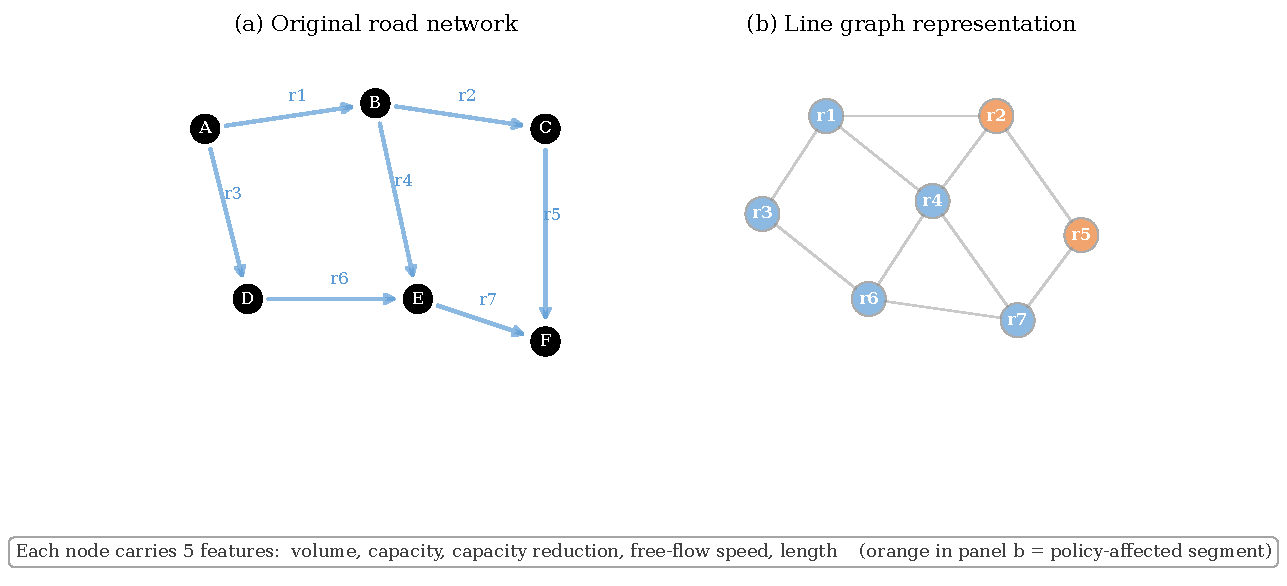
\includegraphics[width=0.95\textwidth]{figures/new/fig31_network_intro.pdf}
 \caption[Paris road network as a directed line graph used by the GNN surrogate]{%
 The Paris road network represented as a directed line graph.\ Each road segment is a node, and edges connect adjacent segments.\ Each node carries five input features describing the segment's traffic state and physical properties.\ The full Paris network contains $31{,}635$ nodes; with 100 graphs in the test set, this gives $3{,}163{,}500$ individual node-level test predictions.\ Adapted from \textcite{natterer2025ml}.}
 \label{fig:network_schematic}
\end{figure}

\section{Contributions}\label{sec:contributions}

\begin{enumerate}
 \item \textbf{A systematic UQ evaluation for a GNN traffic surrogate.}\ Six methods (MC Dropout, seed-ensemble variance, multi-model ensembles, deep ensembles, heteroscedastic regression, CQR) compared on a Paris road-network dataset with $3{,}163{,}500$ node-level test predictions across 100 scenarios.

 \item \textbf{An empirical characterisation of MC Dropout for GNN traffic surrogates.}\ For Trial~8, the pooled (node-level) Spearman $\rho = 0.4820$ at $S = 30$ samples; the mean per-graph $\rho$ is $0.464$ with bootstrap 95\% CI $[0.460, 0.469]$.\ A formal $S$-convergence study confirms that $\rho$ has converged by $S = 30$ (the gain from $S = 30$ to $S = 50$ is only $+1.03\%$).

 \item \textbf{Practical limits of single-architecture ensembles.}\ Five seeded MC Dropout runs raise $\rho$ to $0.4908$; seed ensemble variance gives $\rho = 0.4370$.\ A weighted multi-model ensemble of five trials reaches $\rho = 0.4333$ and $R^2 = 0.5656$, below the best single model.

 \item \textbf{A layered post-hoc calibration framework.}\ Split conformal achieves $\mathrm{PICP}_{90} = 90.02\%$ and $\mathrm{PICP}_{95} = 95.01\%$.\ Regression $\sigma$-scaling with $T = 2.887$ reduces ECE from $0.356$ to $0.034$ ($-90.5\%$) and brings $1\sigma$ coverage from $32.7\%$ to $68.0\%$.\ Adaptive conformal narrows conditional coverage from $[59.0\%, 98.1\%]$ to $[83.7\%, 96.4\%]$.

 \item \textbf{Selective prediction and error detection.}\ Retaining the most confident $50\%$ of predictions reduces MAE by $41.2\%$ to $2.32$ veh/h; AUROC for top-10\% error detection reaches $0.7548$.

 \item \textbf{An empirical observation about freezing the backbone.}\ When the same MSE-trained backbone is reused with three different uncertainty-aware heads, the result depends on whether the backbone is frozen.\ Trial~9 (heteroscedastic head, frozen backbone) is partial-positive at $k_{95} = 2.84$ and $R^2 = 0.4991$; Trial~10 (CQR, backbone unfrozen) is a negative result at $R^2 = 0.4057$ with three of six gates failing; Trial~11, which uses the same CQR head as Trial~10 but freezes the backbone, passes all six gates with $R^2 = 0.5835$, $\mathrm{PICP}_{90} = 89.82\%$ and $\mathrm{PICP}_{95} = 94.91\%$.\ The T10/T11 pair shares head, loss, data, calibration protocol, and learning rate ($5\times10^{-4}$); their single design difference is the backbone-trainability flag.\ The observation is reported within the scope of this thesis and is not claimed as a general principle.

 \item \textbf{A Deep Ensemble baseline.}\ Five independently seeded models reach $R^2 = 0.6841$ ($+14.8\%$ over T8) but a weaker UQ ranking ($\rho = 0.3997$, $k_{95} = 15.18$).\ The Deep Ensemble is the strongest GNN-based point predictor evaluated, while MC Dropout produces the stronger uncertainty ranking; this complementarity is discussed in Chapter~\ref{chapter:discussion}.\ XGBoost on the same five node features (Section~\ref{sec:non_gnn_baselines}) exceeds the Deep Ensemble on point accuracy at $R^2 = 0.7414$.
\end{enumerate}

\section{Thesis Structure}\label{sec:structure}

The five research questions stated above guide the chapter sequence.\ Chapter~\ref{chapter:background} surveys the theoretical foundations.\ Chapter~\ref{chapter:methodology} presents the architecture and the UQ methods used in the thesis.\ Chapter~\ref{chapter:experiments} covers the dataset and the experimental design.\ Chapter~\ref{chapter:results} reports the empirical findings and closes with an illustrative decision framework.\ Chapter~\ref{chapter:discussion} answers the research questions, summarises the primary findings, discusses the freezing-backbone observation, and lists the limitations, threats to validity and future work.\ Chapter~\ref{chapter:conclusion} offers closing remarks, and Appendix~\ref{app:master_table} collects the verified master tables.
